%%%%%%%%%%%%%%%%%%%%%%%%%%%%%%%%%%%%%%%%%
% Beamer Presentation
% LaTeX Template
% Version 1.0 (10/11/12)
%
% This template has been downloaded from:
% http://www.LaTeXTemplates.com
%
% License:
% CC BY-NC-SA 3.0 (http://creativecommons.org/licenses/by-nc-sa/3.0/)
%
%%%%%%%%%%%%%%%%%%%%%%%%%%%%%%%%%%%%%%%%%

%----------------------------------------------------------------------------------------
%	PACKAGES AND THEMES
%----------------------------------------------------------------------------------------

\documentclass{beamer}

\mode<presentation> {

% The Beamer class comes with a number of default slide themes
% which change the colors and layouts of slides. Below this is a list
% of all the themes, uncomment each in turn to see what they look like.

%\usetheme{default}
%\usetheme{AnnArbor}
%\usetheme{Antibes}
%\usetheme{Bergen}
%\usetheme{Berkeley}
%\usetheme{Berlin}
%\usetheme{Boadilla}
%\usetheme{CambridgeUS}
%\usetheme{Copenhagen}
%\usetheme{Darmstadt}
%\usetheme{Dresden}
%\usetheme{Frankfurt}
%\usetheme{Goettingen}
%\usetheme{Hannover}
%\usetheme{Ilmenau}
%\usetheme{JuanLesPins}
%\usetheme{Luebeck}
\usetheme{Madrid}
%\usetheme{Malmoe}
%\usetheme{Marburg}
%\usetheme{Montpellier}
%\usetheme{PaloAlto}
%\usetheme{Pittsburgh}
%\usetheme{Rochester}
%\usetheme{Singapore}
%\usetheme{Szeged}
%\usetheme{Warsaw}

% As well as themes, the Beamer class has a number of color themes
% for any slide theme. Uncomment each of these in turn to see how it
% changes the colors of your current slide theme.

%\usecolortheme{albatross}
%\usecolortheme{beaver}
%\usecolortheme{beetle}
%\usecolortheme{crane}
%\usecolortheme{dolphin}
%\usecolortheme{dove}
%\usecolortheme{fly}
%\usecolortheme{lily}
%\usecolortheme{orchid}
%\usecolortheme{rose}
%\usecolortheme{seagull}
%\usecolortheme{seahorse}
%\usecolortheme{whale}
%\usecolortheme{wolverine}

%\setbeamertemplate{footline} % To remove the footer line in all slides uncomment this line
%\setbeamertemplate{footline}[page number] % To replace the footer line in all slides with a simple slide count uncomment this line

%\setbeamertemplate{navigation symbols}{} % To remove the navigation symbols from the bottom of all slides uncomment this line
}

\usepackage{graphicx} % Allows including images
\usepackage{booktabs} % Allows the use of \toprule, \midrule and \bottomrule in tables
\usepackage{verbatim} % Allows the use of \comment{}
\usepackage{hyperref} % Make Urls Blue
\usepackage{listings} % For code blocks
\hypersetup{
    colorlinks=true,
    linkcolor=blue,
    filecolor=magenta,      
    urlcolor=cyan,
}
 
\urlstyle{same}

\newenvironment{wideitemize}{\itemize\addtolength{\itemsep}{10pt}}{\enditemize}

%----------------------------------------------------------------------------------------
%	TITLE PAGE
%----------------------------------------------------------------------------------------
\title[Research Computing]{Research Computing Tutorial} % The short title appears at the bottom of every slide, the full title is only on the title page

\author{David, Mayara, Sebastian} % Your name
\institute[MIT] % Your institution as it will appear on the bottom of every slide, may be shorthand to save space
{
MIT \\ % Your institution for the title page
\medskip
%\textit{ssteffen@mit.edu} % Your email address
}
\date{\today} % Date, can be changed to a custom date

\begin{document}

\begin{frame}
\titlepage % Print the title page as the first slide
\end{frame}

\begin{frame}
\frametitle{Overview} % Table of contents slide, comment this block out to remove it
\tableofcontents % Throughout your presentation, if you choose to use \section{} and \subsection{} commands, these will automatically be printed on this slide as an overview of your presentation
\end{frame}

\AtBeginSection[]
  {
     \begin{frame}<beamer>
     \frametitle{Workshop Outline}
     \tableofcontents[currentsection]
     \end{frame}
  }

%----------------------------------------------------------------------------------------
%	CODE SNIPPETS
%----------------------------------------------------------------------------------------
\begin{comment}
%------------------------------------------------
\section{First Section} % Sections can be created in order to organize your presentation into discrete blocks, all sections and subsections are automatically printed in the table of contents as an overview of the talk
%------------------------------------------------

\subsection{Subsection Example} % A subsection can be created just before a set of slides with a common theme to further break down your presentation into chunks

\begin{frame}
\frametitle{Paragraphs of Text}
Sed iaculis dapibus gravida. Morbi sed tortor erat, nec interdum arcu. Sed id lorem lectus. Quisque viverra augue id sem ornare non aliquam nibh tristique. Aenean in ligula nisl. Nulla sed tellus ipsum. Donec vestibulum ligula non lorem vulputate fermentum accumsan neque mollis.\\~\\

Sed diam enim, sagittis nec condimentum sit amet, ullamcorper sit amet libero. Aliquam vel dui orci, a porta odio. Nullam id suscipit ipsum. Aenean lobortis commodo sem, ut commodo leo gravida vitae. Pellentesque vehicula ante iaculis arcu pretium rutrum eget sit amet purus. Integer ornare nulla quis neque ultrices lobortis. Vestibulum ultrices tincidunt libero, quis commodo erat ullamcorper id.
\end{frame}

%------------------------------------------------

\begin{frame}
\frametitle{Bullet Points}
\begin{itemize}
\item Lorem ipsum dolor sit amet, consectetur adipiscing elit
\item Aliquam blandit faucibus nisi, sit amet dapibus enim tempus eu
\item Nulla commodo, erat quis gravida posuere, elit lacus lobortis est, quis porttitor odio mauris at libero
\item Nam cursus est eget velit posuere pellentesque
\item Vestibulum faucibus velit a augue condimentum quis convallis nulla gravida
\end{itemize}
\end{frame}

%------------------------------------------------

\begin{frame}
\frametitle{Blocks of Highlighted Text}
\begin{block}{Block 1}
Lorem ipsum dolor sit amet, consectetur adipiscing elit. Integer lectus nisl, ultricies in feugiat rutrum, porttitor sit amet augue. Aliquam ut tortor mauris. Sed volutpat ante purus, quis accumsan dolor.
\end{block}

\begin{block}{Block 2}
Pellentesque sed tellus purus. Class aptent taciti sociosqu ad litora torquent per conubia nostra, per inceptos himenaeos. Vestibulum quis magna at risus dictum tempor eu vitae velit.
\end{block}

\begin{block}{Block 3}
Suspendisse tincidunt sagittis gravida. Curabitur condimentum, enim sed venenatis rutrum, ipsum neque consectetur orci, sed blandit justo nisi ac lacus.
\end{block}
\end{frame}

%------------------------------------------------

\begin{frame}
\frametitle{Multiple Columns}
\begin{columns}[c] % The "c" option specifies centered vertical alignment while the "t" option is used for top vertical alignment

\column{.45\textwidth} % Left column and width
\textbf{Heading}
\begin{enumerate}
\item Statement
\item Explanation
\item Example
\end{enumerate}

\column{.5\textwidth} % Right column and width
Lorem ipsum dolor sit amet, consectetur adipiscing elit. Integer lectus nisl, ultricies in feugiat rutrum, porttitor sit amet augue. Aliquam ut tortor mauris. Sed volutpat ante purus, quis accumsan dolor.

\end{columns}
\end{frame}

%------------------------------------------------
\section{Second Section}
%------------------------------------------------

\begin{frame}
\frametitle{Table}
\begin{table}
\begin{tabular}{l l l}
\toprule
\textbf{Treatments} & \textbf{Response 1} & \textbf{Response 2}\\
\midrule
Treatment 1 & 0.0003262 & 0.562 \\
Treatment 2 & 0.0015681 & 0.910 \\
Treatment 3 & 0.0009271 & 0.296 \\
\bottomrule
\end{tabular}
\caption{Table caption}
\end{table}
\end{frame}

%------------------------------------------------

\begin{frame}
\frametitle{Theorem}
\begin{theorem}[Mass--energy equivalence]
$E = mc^2$
\end{theorem}
\end{frame}

%------------------------------------------------

\begin{frame}[fragile] % Need to use the fragile option when verbatim is used in the slide
\frametitle{Verbatim}
\begin{example}[Theorem Slide Code]
\begin{verbatim}
\begin{frame}
\frametitle{Theorem}
\begin{theorem}[Mass--energy equivalence]
$E = mc^2$
\end{theorem}
\end{frame}\end{verbatim}
\end{example}
\end{frame}

%------------------------------------------------

\begin{frame}
\frametitle{Figure}
Uncomment the code on this slide to include your own image from the same directory as the template .TeX file.
%\begin{figure}
%\includegraphics[width=0.8\linewidth]{test}
%\end{figure}
\end{frame}

%------------------------------------------------

\begin{frame}[fragile] % Need to use the fragile option when verbatim is used in the slide
\frametitle{Citation}
An example of the \verb|\cite| command to cite within the presentation:\\~

This statement requires citation \cite{p1}.
\end{frame}

%------------------------------------------------

\begin{frame}
\frametitle{References}
\footnotesize{
\begin{thebibliography}{99} % Beamer does not support BibTeX so references must be inserted manually as below
\bibitem[Smith, 2012]{p1} John Smith (2012)
\newblock Title of the publication
\newblock \emph{Journal Name} 12(3), 45 -- 678.
\end{thebibliography}
}
\end{frame}
\end{comment}


%----------------------------------------------------------------------------------------
%	PRESENTATION SLIDES
%----------------------------------------------------------------------------------------

\section{Getting Help}
\begin{frame}{Getting Help}
    \begin{itemize}
        \item \textbf{Econ Help:} \url{https://econ-help.mit.edu/}
        \item \textbf{Carl Anderson (E52-311)} \url{econ-support@mit.edu}
        \item \textbf{Slack:} Join \url{mit-econ.slack.com} and message \textbf{\#econ-support}
        \item \textbf{Quickstart:} \url{https://econ-help.mit.edu/kb/quick-start}
        \item \textbf{Overview of Econ clusters:} \url{https://econ-help.mit.edu/kb/rc-systems}
        \item \textbf{Unix Commands:}
        \begin{itemize}
            \item \url{https://econ-help.mit.edu/kb/useful-unix-commands}
            \item \texttt{man $<$command$>$} 
        \end{itemize}
        \item \textbf{Available Modules:} \url{https://econ-help.mit.edu/kb/env-modules}
    \end{itemize}
\end{frame}
%------------------------------------------------

\section{Available Research Computing Systems}
\begin{frame}{Servers and Clusters}
    \begin{itemize}
        \item \textbf{Servers}: each has about has about 1.5TB of RAM and 72 CPUs.
        \begin{itemize}
            \item supply.mit.edu
            \item demand.mit.edu
            \item blackmarket.mit.edu
            \item econometrics.mit.edu
        \end{itemize}
        \item \textbf{Clusters of servers}: High-performance computing.
       \begin{itemize}
            \item reducedform.mit.edu
            \item eosloan.mit.edu ("engaging" - Sloan only)
            \item Host your own: AWS (Amazon), Microsoft Azure, IBM Cloud, Google, other IaaS/SaaS
       \end{itemize}
       \item You connect to servers and clusters the same way, but running code on clusters is slightly different (won't cover today).
 \end{itemize}
\end{frame}
%----------------------------------------------------------------------------------------
\section{Connecting to Computing Systems}
\begin{frame}{Before we begin: MIT Secure Wifi (on campus) \\ or VPN (off campus)}
   \begin{columns}[c]
        \column{.5\textwidth} % Left column and width
        \begin{figure}
        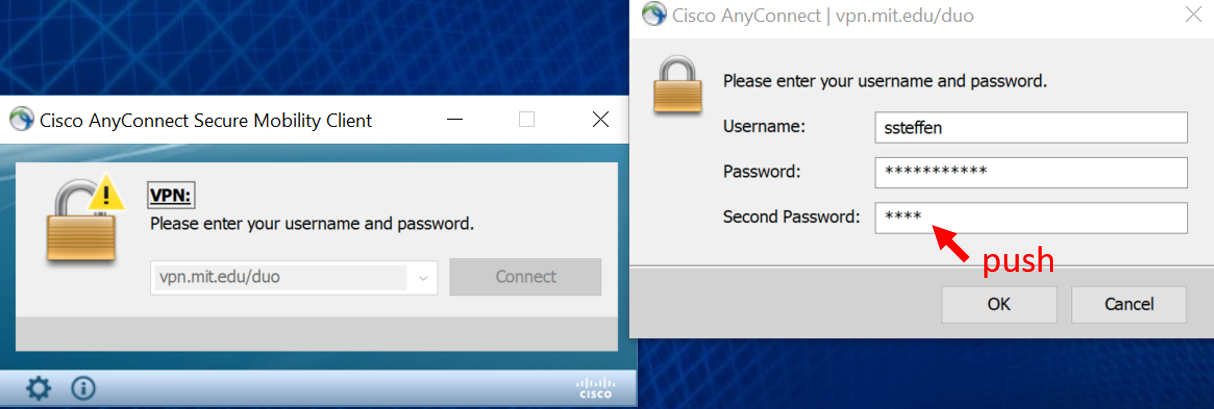
\includegraphics[width=1.0\linewidth]{resources/03_vpn.png}
        \end{figure}
        \column{.5\textwidth} % Right column and width
            \begin{enumerate}
                \item \textbf{Install Cisco AnyConnect:} \url{http://kb.mit.edu/confluence/display/istcontrib/Cisco+AnyConnect+VPN+Landing+Page}
        \item \textbf{Connect to:} \url{vpn.mit.edu/duo} and follow Duo-Authentication steps
            \end{enumerate}
    \end{columns}
\end{frame}
%----------------------------------------------------------------------------------------
\subsection{SSH}
\begin{frame}{How to Connect to MIT Servers}
    \begin{itemize}
        \item \textbf{Connect}: MobaXterm (Windows), Terminal (Mac).
            \begin{itemize}
                \item Mac: \texttt{ssh -X $<$kerberos$>$@$<$hostname$>$.mit.edu}
                \item Windows: Next slide
            \end{itemize}
        \end{itemize}
\end{frame}

\begin{frame}{MobaXterm I}
    \begin{columns}[c]
        \column{.5\textwidth} % Left column and width
        \begin{figure}
        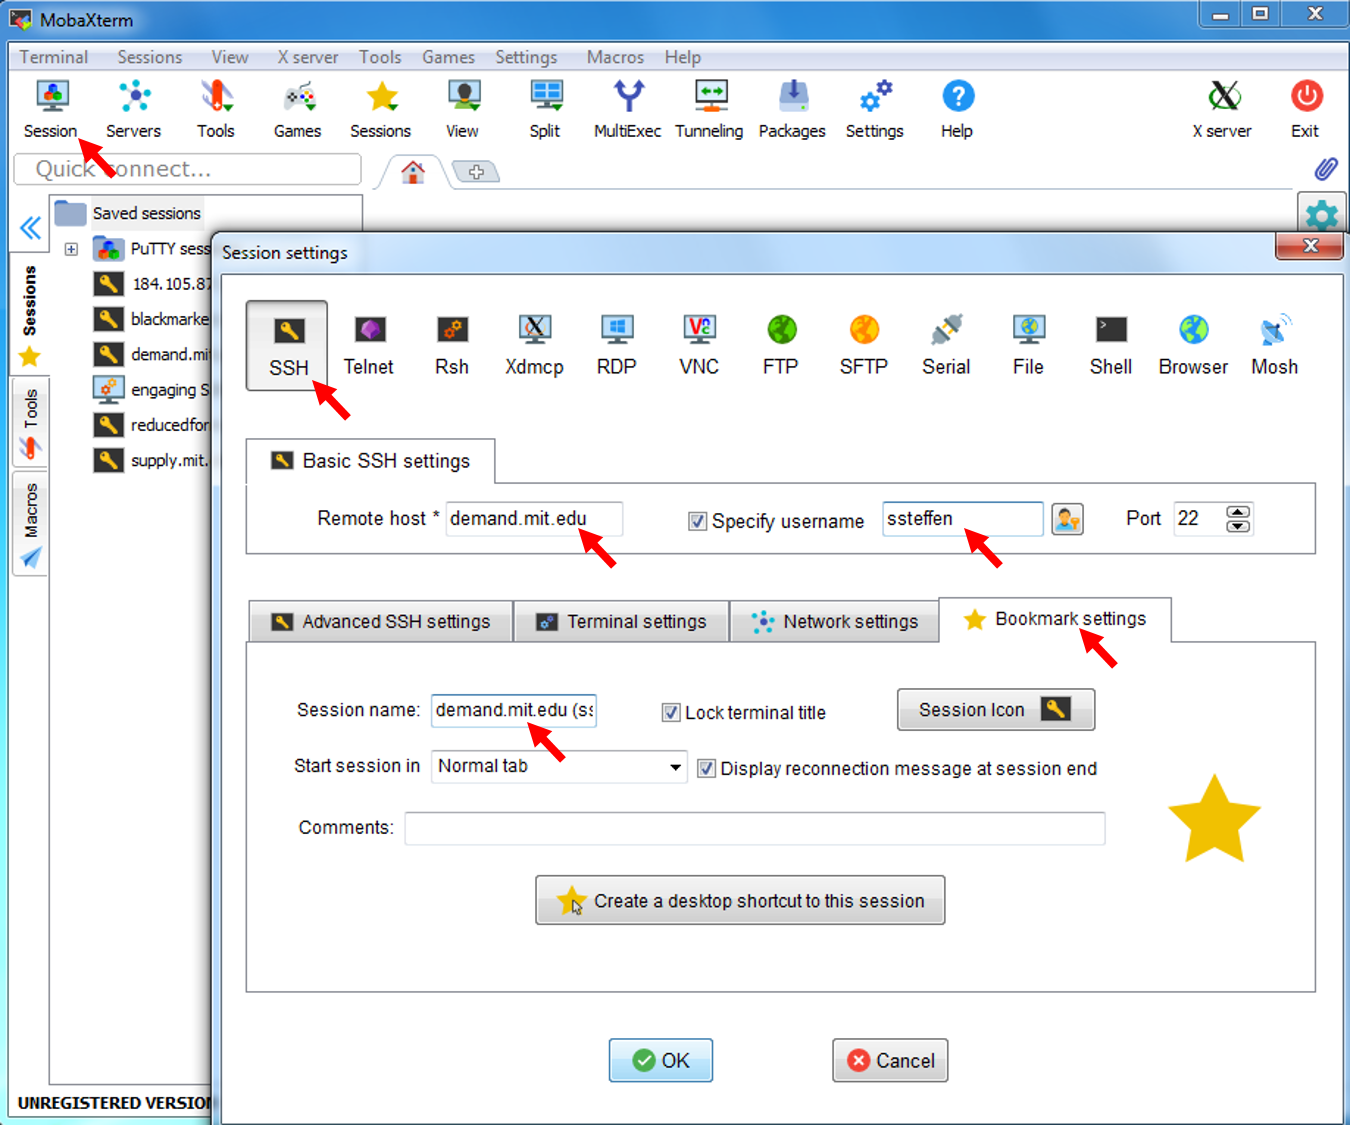
\includegraphics[width=1.0\linewidth]{resources/01_mobaxterm.png}
        \end{figure}
        \column{.5\textwidth} % Right column and width
            \begin{enumerate}
                \item Select \textbf{SSH session}
                \item Enter \textbf{Host address} (i.e. supply.mit.edu) and \textbf{username} (your kerberos)
                \item ...
                \item Profit!
            \end{enumerate}
    \end{columns}
\end{frame}

\subsection{Useful terminal commands}
\begin{frame}{Brief Bash Tutorial}
    \begin{columns}[c] 
        \column{.4\textwidth} % Left column and width
            \textbf{Navigation}
            \begin{itemize}
                \item Get current dir: \texttt{pwd}
                \item Show current dir: \texttt{ls}, \texttt{ls -l}
                \item Move to dir: \texttt{cd $<$PATH$>$}, \texttt{cd $\sim$}(Home), \texttt{cd ..} (Up), \texttt{cd -} (Toggle previous path)
                \item Get help: \texttt{man $<$COMMAND$>$}
            \end{itemize}
        \column{.6\textwidth} % Right column and width
            \textbf{Creation \& Destruction}
            \begin{itemize}
                \item Make a folder: \texttt{mkdir $<$NAME$>$}
                \item Delete a folder: \texttt{rm -r $<PATH>$}
                \item Make a file: \texttt{touch $<$NAME$>$}
                \item Open a file: \texttt{nano $<$PATH$>$ or vim $<$PATH$>$}
                \item View file contents: \texttt{cat $<$NAME$>$}
                \item Delete a file: \texttt{rm $<$PATH$>$}
                \item Copy/Rename a file: \texttt{cp $<$PATH$>$ $<$PATH$>$}
                \item Move a file: \texttt{mv $<$PATH$>$ $<$PATH$>$}
            \end{itemize}
    \end{columns}
\end{frame}

\section{Interacting with MIT Servers}
\subsection{Transfer files}
\begin{frame}{How to Interact with MIT Servers: File transfers}
    \begin{itemize}
        \item To run software on the server, the program you want to run cannot be saved (only) on your local machine - it needs to be accessible by server computers.
        \begin{itemize}
            \item You can use your ECON account for this purpose. Each student with an ECON account has about 200GB of space that can be used for storing data and code (e.g. bbkinghome/mfelix).
        \end{itemize}
       \item Files can be transferred from your local machine to server folders using Secure File Transfer Protocol (SFTP) software.
        \begin{itemize}
             \item Windows: \textbf{MobaXterm}
             \item Mac: \textbf{CyberDuck}. Alternatives: Fetch (download: https://ist.mit.edu/fetch) and FileZilla.
        \end{itemize}
        \item You could also directly mount your ECON folder locally through Finder (Mac) or Windows File System (Windows).
    \end{itemize}
\end{frame}

\subsection{Run code}
\begin{frame}{How to Interact with MIT Servers: Run code}
    \begin{itemize}
        \item \textbf{Interactive mode}
         \begin{itemize}
            \item Windows: From MobaXterm, type xstata, rstudio, python, \dots
             \item Mac: Open \textbf{XQuartz} and type ssh -Y $<$kerberos$>$@$<$server$>$.mit.edu $<$program$>$ (e.g. ssh -Y mfelix@demand.mit.edu stata-mp)
         \end{itemize}
        \item \textbf{Non-interactive mode}
        \begin{itemize}
            \item Same procedure from MobaXterm or from Mac Terminal.
            \item E.g. stata-mp do myfile.do
         \end{itemize}
    \end{itemize}
\end{frame}

\section{Simple exercise: run a .do file}
\begin{frame}{Simple exercise: run a .do file}
\begin{itemize}
    \item Connect to any of the servers
    \item cd /bbkinghome/mfelix/workshop
    \item ls
    \item stata-mp -b do workshop\_exercise.do
\end{itemize}
\end{frame}  
%----------------------------------------------------------------------------------------

\begin{frame}{Screen}
    \begin{itemize}
        \item The screen command creates persistent, virtual terminal shells that keep running even when you leave.
        \item \textbf{Attach a screen:} \texttt{screen -S $<$name$>$}
        \item \textbf{List your screens:} \texttt{screen -ls}
        \item \textbf{Detach a screen} \texttt{Ctrl+A, D}
        \item \textbf{Reattach a screen:} \texttt{screen -r}
        \item \textbf{Learn more:} \texttt{man screen}
    \end{itemize}
\end{frame}

\begin{frame}{Getting Help - Again!}
    \begin{itemize}
        \item \textbf{Econ Help:} \url{https://econ-help.mit.edu/}
        \item \textbf{Carl Anderson (E52-311)} \url{econ-support@mit.edu}
        \item \textbf{Slack:} Join \url{mit-econ.slack.com} and message \textbf{\#econ-support}
        \item \textbf{Overview of Econ clusters:} \url{https://econ-help.mit.edu/kb/rc-systems}
        \item \textbf{Unix Commands:}
        \begin{itemize}
            \item \url{https://econ-help.mit.edu/kb/useful-unix-commands}
            \item \texttt{man $<$command$>$} 
        \end{itemize}
        \item \textbf{Available Modules:} \url{https://econ-help.mit.edu/kb/env-modules}
        \item \textbf{Sloan Engaging:} \url{https://wikis.mit.edu/confluence/display/sloanrc/Engaging+Platform}
    \end{itemize}
\end{frame}
%----------------------------------------------------------------------------------------

\begin{frame}
\Huge{\centerline{Thank You!}} \\
\bigskip
\bigskip
\normalsize{\centerline{Please email feedback to ssteffen@mit.edu.}}
\end{frame}
%----------------------------------------------------------------------------------------

\section{Appendix}
\begin{frame}{Cluster Etiquette}
    \begin{itemize}
        \item Be a \textbf{Good Netizen}: 
        \begin{itemize}
            \item DO cancel stale jobs: scancel <JOB\_ID>
            \item DO set reasonable cpu, time parameters.
            \item DON'T run multiple interactive sessions at once.
            \item DON'T submit too many batch jobs at once (try job arrays).
            \item Up-Arrow to recall history of commands, Tab to Autocomplete.
            \item Only install things for yourself (i.e. \texttt{pip install --user pandas}).
            \item Don't clutter random (i.e. root) paths - double-check where you save your stuff.
            \item Don't try to run stuff in the reducedform login node - it's only able to handle redirecting your programs to the (very powerful) cluster. \href{https://econ-help.mit.edu/kb/useful-rf-command}{There are special simplified commands.}
        \end{itemize}
    \end{itemize}
\end{frame}
%----------------------------------------------------------------------------------------

\begin{frame}{Your Turn I: Bash Exercise}
    \begin{itemize}
        \item Create a file inside a new folder and write in it. 
        \item Move the file to your home directory. 
        \item Create a renamed copy of the file.
        \item Show files sorted by modification time. 
        \item Show file contents.
    \end{itemize}
\end{frame}  
%----------------------------------------------------------------------------------------

\begin{frame}{Solution I: Bash Exercise}
    \begin{itemize}
        \item \texttt{mkdir SBTC\_project}
        \item \texttt{cd SBTC\_project (or cd !\$)}
        \item \texttt{touch import\_ad2013.py}
        \item \texttt{vi import\_ad2013.py}
        \item \texttt{I (insert mode), "Nice.", $<$ESC$>$ (normal mode), :x! (save \& quit)}
        \item Better: \texttt{cat $>$import\_ad2013.py "Nice." <Ctrl+D> (save \& quit)}
        \item \texttt{mv import\_ad2013.py $\sim$/import\_ad2013.py}
        \item \texttt{cp import\_ad2013.py import\_ss2019.py}
        \item \texttt{cd ..}
        \item \texttt{ls -t -l}
        \item \texttt{cat import\_ad2013.py import\_ss2019.py}
    \end{itemize}
\end{frame}
%----------------------------------------------------------------------------------------

\begin{frame}{Useful Bash Stuff to know [Optional]}
    \begin{itemize}
        \item Bash is one of many different shell programming languages. It was first released in 1989.
        \item \textbf{Set shortcuts:} \texttt{alias ..="cd .."}
        \item \texttt{!\$} refers to the previous command's argument.
        \item Google more cool \href{https://unix.stackexchange.com/questions/159513/what-are-the-shells-control-and-redirection-operators}{stuff}: \texttt{screen}, \texttt{grep}, operators like \texttt{|}, \texttt{>}, ...
        \item[]
        \item Instead of directly writing bash commands in the terminal, you can also submit commands via a (bash) script (kind of like a stata .do file).
        \item Example: 
            \begin{itemize}
                \item Create a file and write: \texttt{\#!/bin/bash [linebreak] echo \$PWD}
                \item Make file executable: \texttt{chmod u+x $<$file\_name$>$}
                \item Run it: \texttt{bash $<$file\_name$>$}
            \end{itemize}
    \end{itemize}
\end{frame}
%----------------------------------------------------------------------------------------

\begin{frame}{Upload files to a Cluster: FTP [Optional]}
    \begin{itemize}
        \item \textbf{FTP:} Protocol to transfer files. 
        \item Again, possible via terminal (and command line), but visual clients are more convenient.
        \item Cyberduck (Mac)
        \item MobaXterm (Windows)
        \item[]
        \item A company sends you an ftp link with username and password to their data. Set up a screen connection (to prevent shutdown due to inactivity):
    \end{itemize}
    \begin{verbatim}
        screen -S ftp \\
        wget -m --user=$<$username$>$ --password=$<$password$>$ $<$ftp\_address$>$
    \end{verbatim}
\end{frame}
%----------------------------------------------------------------------------------------

\begin{frame}{Interactive Sessions}
    \begin{itemize}
        \item For easy/early data exploration that does not require large amount of resources.
        \item 'Normal' UI for your program of choice: xstata, rstudio, python, matlab, ...
        \item Windows: just type program in MobaXTerm terminal
        \item Mac: need to run XQuartz (for X-11, i.e. graphics, forwarding).
        \item \textbf{In X-Quartz:} \texttt{ssh -Y $<$kerberos$>$@$<$cluster$>$.mit.edu $<$program$>$}
    \end{itemize}
\end{frame}
%----------------------------------------------------------------------------------------

\begin{frame}{Change Program Version [Optional]}
    \begin{itemize}
        \item \textbf{See what other modules are available:}  \texttt{module avail}
        \item \textbf{See currently loaded modules:} \texttt{module list}
        \item \textbf{Load module:} \texttt{module load $<$module$>$}
        \item Example I: Load Python 3 instead of default Python 2 (\href{https://pythonclock.org/}{which retires in less than a year!})
        \begin{itemize}
            \item View 'software collections': \texttt{ scl -l}
            \item \texttt{scl enable python33 bash} 
        \end{itemize}
        \item Example II: Load older Stata
        \begin{itemize}
            \item \texttt{module load stata/13}
        \end{itemize}
        \item \textbf{Caveat:} On reducedform nothing is preloaded. Need to specify everything in bash file.
    \end{itemize}
\end{frame}
%----------------------------------------------------------------------------------------

\begin{frame}{ReducedForm - PBS Job Scheduler}
    \begin{itemize}
        \item reducedform is a HPC cluster with a dedicated job scheduler - Portable Batch System (PBS).
        \item MIT Sloan's engaging uses SLURM, a slightly different job scheduler.
        \item Job Scheduler automatically schedules jobs and allocates resources efficiently.
        \item[]
        \item Need to submit bash file with info on what script to run, what modules (i.e. Python, R, CRAN, another file you wrote) are required to run it, as well as job parameters (partition, time, CPUs, messages, ...)
    \end{itemize}
\end{frame}
%----------------------------------------------------------------------------------------

\begin{frame}[label=BashFileSlideBack]{Submitting First ReducedForm 'Batch Job' via bash file [Optional]}
    \begin{itemize}
        \item bash file, which specifies all parameters, files, and \textbf{modules}: \hyperlink{BashFileSlide}{\beamergotobutton{Example}}
        \item \textbf{Submit a batch job:} \texttt{qsub job\_file.sh (sbatch)}
        \item Check on job: \texttt{checkjob} 
        \item Delete a job: \texttt{qdel job\_id (scancel)}
        \item Show all jobs: \texttt{qstat (squeue)}
        \item List available modules: \texttt{module list}, \texttt{module avail}, \texttt{scl -l}
        \item \texttt{scl enable python33 bash}
        \item Break out of execution: \texttt{Command + D}
        \item easy (interactive) alternative for \href{https://econ-help.mit.edu/kb/matlab-stata-rf}{stata, matlab}: \texttt{statajob}, \texttt{matlabjob}
    \end{itemize}
\end{frame}
%----------------------------------------------------------------------------------------

\begin{comment}
\begin{frame}{Your Turn II}
    \begin{itemize}
        \item Run an interactive Stata, and Rstudio session.
        \item Copy/Write and save a bash script.
        \item Upload it to the cluster.
        \item Kill both jobs.
        \item Delete everything.
    \end{itemize}
\end{frame}
%----------------------------------------------------------------------------------------

\begin{frame}{Solution II}
    \begin{itemize}
        \item Drag \& Drop to upload.
        \item \texttt{qdel $<$job_id$>$} 
        \item \texttt{rm import\_ad2013.py}
        \item \texttt{rm -d SBTC\_project}
    \end{itemize}
\end{frame}
\end{comment}
%----------------------------------------------------------------------------------------

\begin{frame}{Install Anaconda for Python Virtual Environments [Optional]}
    \begin{itemize}
        \item \texttt{curl -O https://repo.continuum.io/archive/Anaconda3-5.0.1-Linux-x86\_64.sh}
        \item \texttt{bash Anaconda3-5.0.1-Linux-x86\_64.sh}
        \item \texttt{source $\sim$/.bashrc}
        \item Jupyter Notebooks can be run via \href{https://wikis.mit.edu/confluence/display/sloanrc/Text+Editors+and+IDEs}{tunneling on Engaging}. 
    \end{itemize}
\end{frame}
%----------------------------------------------------------------------------------------

\begin{frame}{Tunneling [Optional]}
    \begin{columns}[c]
    \column{.5\textwidth} % Left column and width
    \begin{figure}
    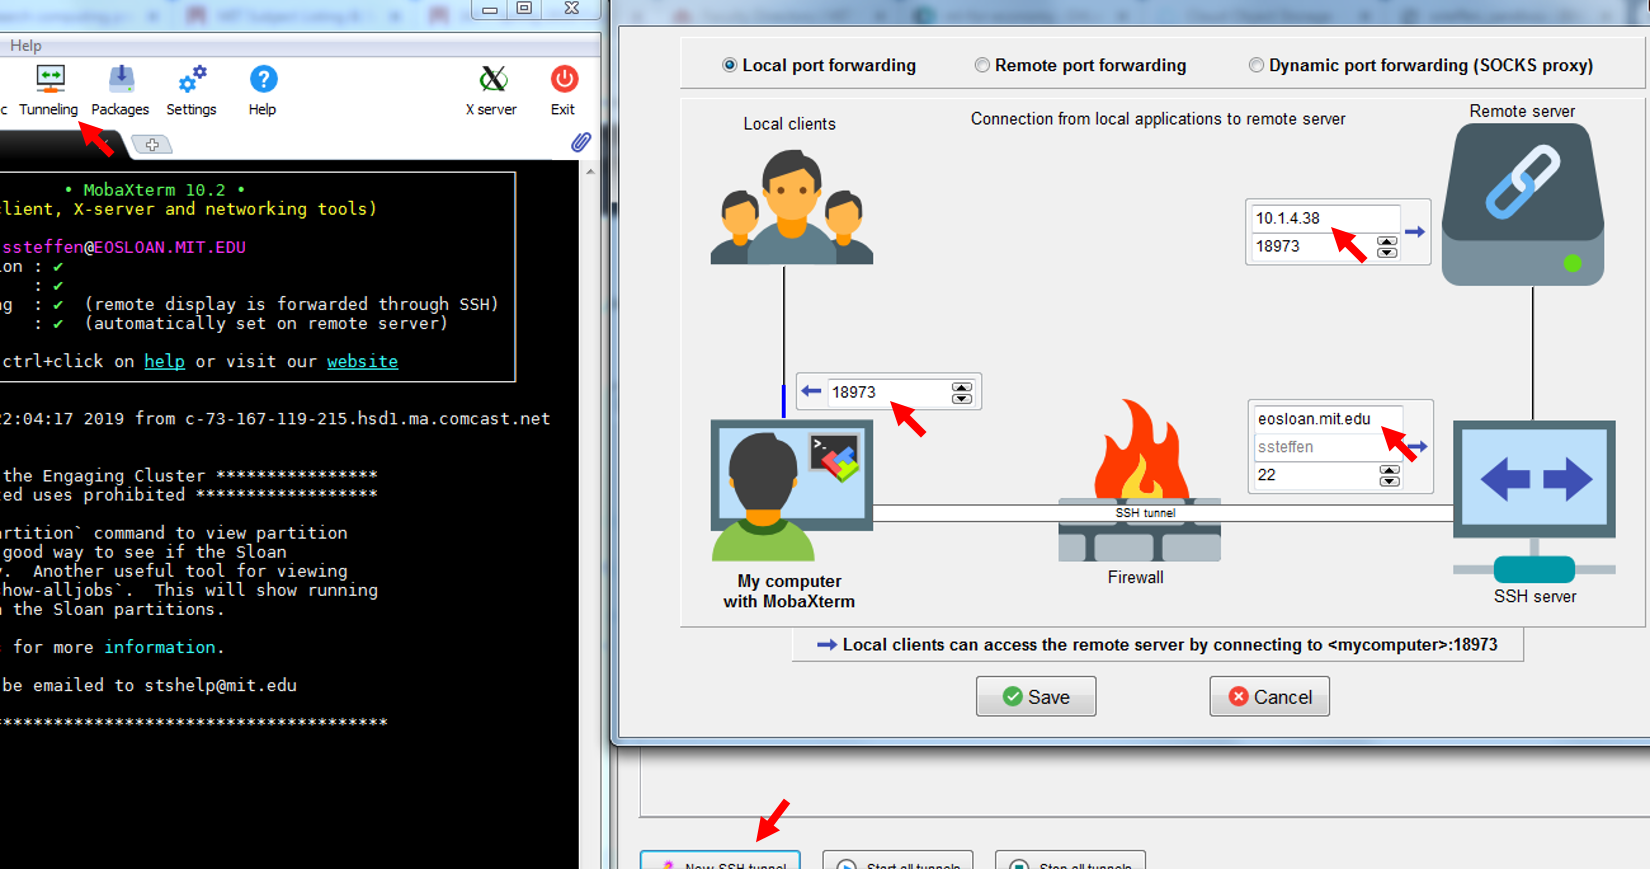
\includegraphics[width=1.0\linewidth]{resources/02_mobaxterm.png}
    \end{figure}
    \column{.5\textwidth} % Right column and width
        \begin{enumerate}
            \item Select \textbf{SSH session}
            \item Enter \textbf{Host address} (i.e. supply.mit.edu) and \textbf{username} (your kerberos)
            \item ...
            \item Profit!
        \end{enumerate}
\end{columns}
\end{frame}

%----------------------------------------------------------------------------------------

\begin{frame}{Loose Ends I: Storage, Git, Access control [Optional]}
    \begin{itemize}
        \item Dropbox was founded in 2007 by MIT students.
        \item $\Rightarrow$ Unlimited Dropbox storage for all MIT students! \href{https://ist.mit.edu/dropbox}{Link}
        \item[]
        \item Quick and easy git guide: \href{http://rogerdudler.github.io/git-guide/}{Link}
        \item Can download 'Github Desktop' GUI to avoid terminal commands: \href{https://desktop.github.com/}{Link}
        \item[] 
        \item To collaborate on cluster: make groups, assign them folders, and change access rights: \href{https://ss64.com/bash/chmod.html}{Link}
        \item Make a group: \texttt{groupadd $<$group$>$}
        \item Add collaborators to groups: \texttt{usermod -a -G $<$group$>$ $<$user$>$}
        \item Change a folder's owner to group: \texttt{chgrp -hR $<$group$>$ $<$folder$>$}
        \item Give read, write, execute rights to group members: \texttt{chmod 770}
    \end{itemize}
\end{frame}
%----------------------------------------------------------------------------------------

\begin{frame}{Unsolicited, Biased Opinions - Languages}
    \begin{itemize}
        \item Stata: 
        \begin{itemize}
            \item seductively simple and powerful.
            \item not a real programming language.
            \item has no/slow development for modern methods and awful graphics.
        \end{itemize}
        \item R
        \begin{itemize}
            \item excellent hybrid between real programming language, economics, data science.
            \item okay learning curve
            %\item best packages: \texttt{dplyr}, \texttt{ggplot2}
        \end{itemize}
        \item Python
        \begin{itemize}
            \item real programming language, can do anything.
            \item okay learning curve
            %\item best packages: \texttt{pandas}, \texttt{numpy}, \texttt{scikit-learn}
        \end{itemize}
        \item Matlab
        \begin{itemize}
            \item good at optimization.
            \item only used a little bit in Econ and Engineering.
        \end{itemize}
    \end{itemize}
\end{frame}

%----------------------------------------------------------------------------------------

\begin{frame}[label=BashFileSlide]{PBS Job [Optional]}
    \begin{verbatim}
        \#!/bin/bash \\
        \#PBS -N MyJob \\
        \#PBS -l mem=12G,walltime=2:00:00,nodes=1:ppn=1 \\
        \#PBS -m be \\
        \#PBS -M $<$email$>$ \\
        \\
        python $<$script.py$>$
    \end{verbatim}
    See more here: \href{https://econ-help.mit.edu/kb/advanced-batch-usage}{Link} \\
    \hyperlink{BashFileSlideBack}{\beamergotobutton{back}}
\end{frame}
%----------------------------------------------------------------------------------------

\begin{frame}{SLURM Parallel Job [Optional]}
    \begin{verbatim}
    \#!/bin/bash \\
    \#SBATCH -a 2016-2018
    \#SBATCH --cpus-per-task=2
    \#SBATCH --mem-per-cpu=20GB
    \#SBATCH --time=2-00:00:00
    \#SBATCH --partition=sched\_mit\_sloan\_batch
    \#SBATCH --mail-type=BEGIN,END,FAIL
    \#SBATCH --mail-user=ssteffen@mit.edu
    \\
    python $<$script.py$>$ \$SLURM\_ARRAY\_TASK\_ID
    \end{verbatim}
    \hyperlink{BashFileSlideBack}{\beamergotobutton{back}}
\end{frame}
%----------------------------------------------------------------------------------------

\end{document}